
\chapter{Examples for this Template}
\section{Citations}
Cite stuff from the .bib file. 

Cite in text \cite{CostantiniPSP}, Cite with brackets \citep{Schneider2021b}, cite multiple publications from the same authors \cite{Schneider2021b,Schneider2021a} / \citep{Schneider2021b,Schneider2021a} or different \citep{Schneider2021b,CostantiniPSP} / \cite{Schneider2021b,CostantiniPSP}. 

Cite a specific page:  \cite[see][p. 42]{Schneider2021b}, or chapter \cite[compare ][Ch. 3]{Schneider2021a} 

\section{Foot notes}
The end of internet can be visited\footnote{\url{http://endoftheinternet.com/}}. 
Or choose your own number \footnote[42]{Why would you do this?}.

\section{Strike out}

\sout{You can strike out text...}
\section{Todo marker}

You can simply write stuff in red \todo{to quickly note work in progress}.

\section{Abbreviations} 
You can use the defined acronyms like this: when used the first time: Full (Short) \ac{SAR}. When used the second time: SHORT \ac{SAR}. To use plural \acp{SAR}. Full only: \acl{SAR}
More info: \url{https://ctan.net/macros/latex/contrib/acronym/acronym.pdf}

\section{Equations} 

Inline: $a^2+b^2=c^2$.

\begin{align}
a^2+b^2-c^2&=0\\
a^2+b^2&=c^2 \label{eq:pyth}\\
\sqrt{a^2+b^2}&=c
\end{align}

You can refer to lines by label: Eq. (\ref{eq:pyth})

\section{Algorithms and pseudocode}
Using usepackage\{algpseudocode\}
\\

\begin{algorithmic}
	\State $i \gets 10$
	\If{$i\geq 5$} 
	\State $i \gets i-1$
	\Else
	\If{$i\leq 3$}
	\State $i \gets i+2$
	\EndIf
	\EndIf 
\end{algorithmic}

\section{Tables} 
You can refer to a Table CHAPTER.NUMBER: Table \ref{tab:example1}. You find nice examples of Tables online \footnote{\url{https://tex.stackexchange.com/questions/112343/beautiful-table-samples}}.
\begin{table}[!hb]
	\centering
	\begin{tabular}{rrrrrrrr} \toprule
		{$m$} & {$\Re\{\underline{\mathfrak{X}}(m)\}$} & {$-\Im\{\underline{\mathfrak{X}}(m)\}$} & {$\mathfrak{X}(m)$} & {$\frac{\mathfrak{X}(m)}{23}$} & {$A_m$} & {$\varphi(m)\ /\ ^{\circ}$} & {$\varphi_m\ /\ ^{\circ}$} \\ \midrule
		1  & 16.128 & +8.872 & 16.128 & 1.402 & 1.373 & -146.6 & -137.6 \\
		2  & 3.442  & -2.509 & 3.442  & 0.299 & 0.343 & 133.2  & 152.4  \\
		3  & 1.826  & -0.363 & 1.826  & 0.159 & 0.119 & 168.5  & -161.1 \\
		4  & 0.993  & -0.429 & 0.993  & 0.086 & 0.08  & 25.6   & 90     \\ \midrule
		5  & 1.29   & +0.099 & 1.29   & 0.112 & 0.097 & -175.6 & -114.7 \\
		6  & 0.483  & -0.183 & 0.483  & 0.042 & 0.063 & 22.3   & 122.5  \\
		7  & 0.766  & -0.475 & 0.766  & 0.067 & 0.039 & 141.6  & -122   \\
		8  & 0.624  & +0.365 & 0.624  & 0.054 & 0.04  & -35.7  & 90     \\ \midrule
		9  & 0.641  & -0.466 & 0.641  & 0.056 & 0.045 & 133.3  & -106.3 \\
		10 & 0.45   & +0.421 & 0.45   & 0.039 & 0.034 & -69.4  & 110.9  \\
		11 & 0.598  & -0.597 & 0.598  & 0.052 & 0.025 & 92.3   & -109.3 \\ \bottomrule
	\end{tabular}
\caption{A Table}
\label{tab:example1}
\end{table}

\begin{table*}[!b]
	\begin{centering}
		\begin{adjustbox}{max width=\textwidth}
			\begin{tabular}{llcccccl}
				\toprule
				& & & & & \multicolumn{2}{c}{Attributes} &  \\ \cline{6 - 7} \rule{0pt}{2.5ex}
				Data Set & Split & \# Points [Mio] & Area [km$^2$] & Density [pts/m$^2$] & LiDAR & Color & Classes \\
				\toprule
				
				\multirow{3}{*}{\textbf{V3D}} &
				\multirow{3}{*}{\shortstack[l]{train \\ test}} &
				\multirow{3}{*}{\shortstack[l]{0.754 \\ 0.412}} &
				\multirow{3}{*}{\shortstack[l]{0.084  \\ 0.046}} &
				\multirow{3}{*}{3}  &
				\multirow{3}{*}{\shortstack[l]{Intensity, \\ Echo Number, \\\# Echos}} &
				\multirow{3}{*}{CIR} &
				\multirow{3}{*}{\shortstack[l]{\textit{Powerline}, \textit{Low Vegetation}, \textit{Impervious Surface}, \\ \textit{Car}, \textit{Fence/Hedge}, \textit{Roof}, \textit{Fa\c{c}ade}, \textit{Shrub}, \textit{Tree} }} \\
				& & & & &  & & \\
				& & & & & & & \\
				\midrule	
				
				\multirow{3}{*}{\textbf{H3D}} &
				\multirow{3}{*}{\shortstack[l]{train \\ \rule{0pt}{0.0001cm} \\ test}} &
				\multirow{3}{*}{\shortstack[l]{73.909 \\ \rule{0pt}{0.0001cm} \\ 51.745}} &
				\multirow{3}{*}{\shortstack[l]{0.030 \\ \rule{0pt}{0.0001cm} \\ 0.031}} &
				\multirow{3}{*}{3}  &
				\multirow{3}{*}{\shortstack[l]{Reflectance, \\ Echo Number, \\\# Echos}} &
				\multirow{3}{*}{RGB} &
				\multirow{3}{*}{\shortstack[l]{\textit{Low Vegetation}, \textit{Impervious Surface}, \textit{Vehicle},  \\ \textit{Urban Furniture}, \textit{Roof}, \textit{Fa\c{c}ade}, \textit{Shrub}, \textit{Tree}, \\ \textit{Soil/Gravel}, \textit{Vertical Surface}, \textit{Chimney} }} \\
				& & & & &  & & \\
				& & & & & & & \\
				\midrule	
				
				\multirow{3}{*}{\textbf{S3D}} &
				\multirow{3}{*}{\shortstack[l]{train \\ \rule{0pt}{0.0001cm} \\ test}} &
				\multirow{3}{*}{\shortstack[l]{38.511 \\ \rule{0pt}{0.0001cm} \\ 40.417}} &
				\multirow{3}{*}{\shortstack[l]{1.819 \\ \rule{0pt}{0.0001cm} \\ 2.179}} &
				\multirow{3}{*}{3}  &
				\multirow{3}{*}{\shortstack[l]{Intensity, \\ Echo Number, \\\# Echos}} &
				\multirow{3}{*}{RGB} &
				\multirow{3}{*}{\shortstack[l]{\textit{Urban Furniture}, \textit{Ground},  \textit{Building},  \textit{Tree} }} \\
				& & & & &  & & \\
				& & & & & & & \\
				
				\bottomrule
			\end{tabular}
		\end{adjustbox}
		\caption{Features used as input for the RF classifier.}
		\label{tab:comparison}
		%\end{adjustbox}
	\end{centering}
\end{table*}

\section{Figures}   

\begin{figure}[!hb]
	\centering 
	\includegraphics[width=0.45\linewidth,trim={2cm 6cm 0cm 8cm},clip]{figures/example1/figure} %  trim={<left> <lower> <right> <upper>}
	\fbox{
		\includegraphics[width=0.45\linewidth,trim={2cm 6cm 0cm 8cm},clip]{figures/example1/figure} }%  trim={<left> <lower> <right> <upper>} 
	\caption{Double, including frame}
	\label{fig:double_example1}
\end{figure}



\begin{figure}[ht]
	\begin{subfigure}{.5\textwidth}
		\centering
		% include first image
	\includegraphics[width=1\linewidth,trim={2cm 6cm 0cm 8cm},clip]{figures/example1/figure} %  trim={<left> <lower> <right> <upper>}	
		\caption{Put your sub-caption here}
		\label{fig:sub-first}
	\end{subfigure}
	\begin{subfigure}{.5\textwidth}
		\centering
		% include second image
	\includegraphics[width=1\linewidth,trim={2cm 6cm 0cm 8cm},clip]{figures/example1/figure} %  trim={<left> <lower> <right> <upper>}	
		\caption{Put your sub-caption here}
		\label{fig:sub-second}
	\end{subfigure}
	\caption{Put your caption here}
	\label{fig:fig}
\end{figure}

\begin{figure}[!hb]
	\centering
	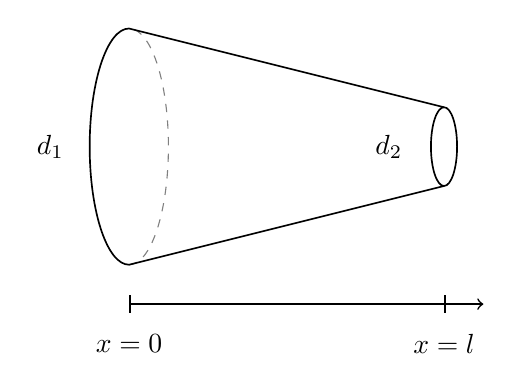
\begin{tikzpicture}
	\draw[dashed,color=gray] (0,0) arc (-90:90:0.5 and 1.5);% right half of the left ellipse
	\draw[semithick] (0,0) -- (4,1);% bottom line
	\draw[semithick] (0,3) -- (4,2);% top line
	\draw[semithick] (0,0) arc (270:90:0.5 and 1.5);% left half of the left ellipse
	\draw[semithick] (4,1.5) ellipse (0.166 and 0.5);% right ellipse
	\draw (-1,1.5) node {$\varnothing d_1$};
	\draw (3.3,1.5) node {$\varnothing d_2$};
	\draw[|-,semithick] (0,-0.5) -- (4,-0.5);
	\draw[|->,semithick] (4,-0.5) -- (4.5,-0.5);
	\draw (0,-1) node {$x=0$};
	\draw (4,-1) node {$x=l$};
	\end{tikzpicture}
	\caption{TikZ example: The graphic shows a truncated cone. The diameter of the cone changes from $d_1$ to $d_2$ along the x-direction.}
	\label{fig:exampletikz}
\end{figure}
\subsection{Referencing Figures}
Reference a Figure, the number will be CHAPTER.NUMFIG Figure \ref{fig:single_example1}
\begin{figure}[!b]
	\centering 
	\includegraphics[width=0.7\linewidth,trim={2cm 6cm 0cm 8cm},clip,, angle =42 ]{figures/example2/figure} %  trim={<left> <lower> <right> <upper>}
	\caption{You can Rotated and crop an image in-line}
	\label{fig:single_example1}
\end{figure}


\FloatBarrier

